%!TEX root = ../thesis.tex

\todo{Example with a large mass companion? and/or \snr{}.}

\section{Results}
\label{sec:chi2_results}

%!TEX root = ../thesis.tex

\begin{table*}
      \centering
      \begin{threeparttable}
          \caption{Input and recovered parameters on simulations and an observation when applying a single (\(\rm C^1\)) and binary (\(\rm C^2\)) models. The \logg{} and metallicity were fixed at \(\logg{}_1 = 4.50\), \(\logg{}_2=5.0\) and \feh{}=0.0 equally for both components. Gaussian noise was added to both simulations with a \snr{} of 150. Here \(m\) and \(n\) are the number of data points and parameters used in each model.}

          \begin{tabular}{c | *3c | *3c | *3c}
              \toprule
              & \multicolumn{3}{c|}{Simulation 1} & \multicolumn{3}{c|}{Simulation 2} & \multicolumn{3}{c}{Observed {HD 211847}} \\
              \midrule
          & Input & \multicolumn{2}{c|}{Recovered} & Input & \multicolumn{2}{c|}{Recovered} & Expected & \multicolumn{2}{c}{Recovered} \\
          & & \(C^1\) & \(C^2\) & & \(C^1\) & \(C^2\) & & \(C^1\)  & \(C^2\) \\
          \midrule
          \(\teffsub{1}\) & 5\,800 & 5\,800 & 5\,800 & 5\,700 & 5\,800 & 5\,700 & \(5\,715 \pm 24\) & 5\,900 & 5\,800\\
          \(\teffsub{2}\) & 4\,000 & -- & 3\,800 & 3\,200 & -- & 3\,100 & \(\sim\)3\,200 & -- & >3\,800\tnote{a}\\
          \({rv}_1\) & 0 & 0.1 & 0 & 6.6 & 6.6 & 6.6 & \(6.6 \pm 0.3\) & 7& 7.6 \\
          \({rv}_2\) &  10 & -- & 9.8 & 0.5 & -- &  -1& \(0.5 \pm 2\) & -- &-12.6\\
          \midrule
          \(R_1/R_2\)& 2.57 & -- & 2.71& 3.16 & - & 3.27 & 3.16 & -- & <2.71\tnote{a}\\
          \(\rm F_2/F_1\)& 0.084 & -- & 0.066 & 0.030 & -- & 0.026 & 0.030 & -- & >0.066\tnote{a}\\
          \(m\) & - & 3\,072 & 3\,072 & -- & 3\,072 & 3\,072 & -- & 2\,612 & 2\,612\\
          \(n\) & - & 2 & 4 & -- & 2 & 4 & -- & 2 & 4\\
          \textchisquared& -- & 4\,978 & 3\,792 & -- & 3\,746 & 3\,630  & -- & 37\,688 & 33\,860\\
          \(\chisquared_{red}\) & -- & 1.62 & 1.24 & -- & 1.22 & 1.18 & -- & 21.3 & 19.2\\
          {BIC} & -- & -20\,145 & -22\,315 & -- & -21\,477 & -21\,377& -- & 18\,281 & 14\,468\\
          \bottomrule
        \end{tabular}\label{tab:example_params}
        \begin{tablenotes}
            \item [a] {At the arbitrary upper limit for companion temperature grid (3\,800\K{}).}
        \end{tablenotes}
    \end{threeparttable}
\end{table*}


\begin{figure*}
    \centering
    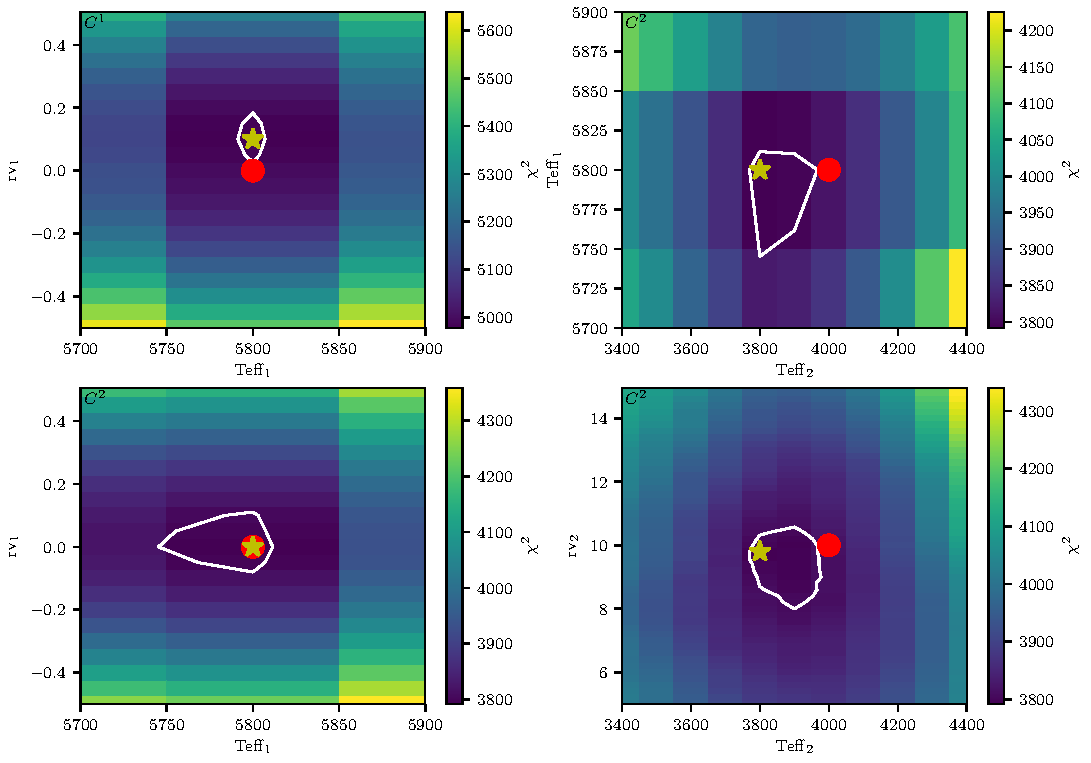
\includegraphics[width=0.7\linewidth]{figures/companion_recovery/Mdwarf_pcolors}
    \caption[\textchisquared{} contour for companion recovery of a simulated Sun - M-dwarf binary.]{\textchisquared{} results for companion recovery of a simulated binary observation of a Sun-like star (\(\teffsub{1}=5800\)\K{}) with an M-dwarf companion (\(\teffsub{2}=4000\)\K{}).
        The top right plot shows the application of a single component model (\(C^1\)) while the other three are using a binary model (\(C^2\)).
        Both left hand panels show the distribution of host temperature and host {RV}.\@ The top right panel shows the distribution for host and companion temperature, and the bottom right the companion temperature and radial velocity.
        The red circle and yellow star indicate the location of the simulation input and recovered parameters respectively.
        The white line shows a 3-\(\sigma\) confidence level about the minimum \textchisquared{} solution grid point.
        Each box is centred on the parameter values and shows the grid resolution.}
    \label{fig:Mdwarf_contours}
\end{figure*}

\begin{figure*}
    \centering
    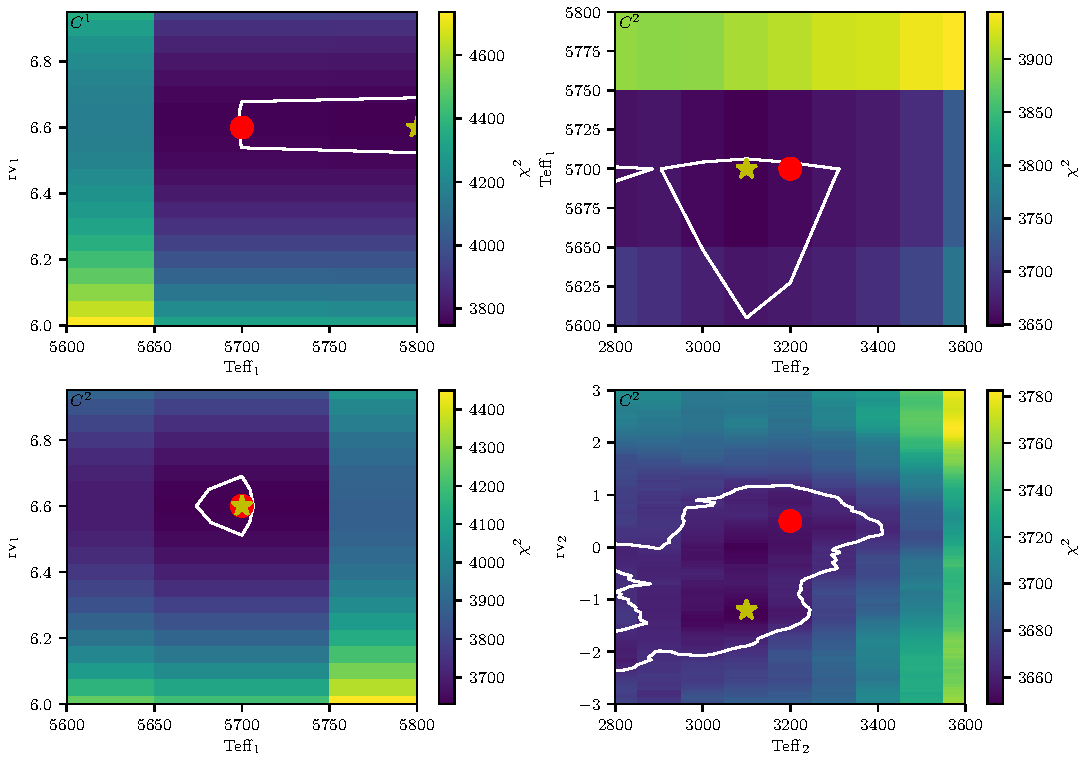
\includegraphics[width=0.7\linewidth]{figures/companion_recovery/HD211847_example_pcolors}
    \caption[\textchisquared{} contour for companion recovery of a simulated observation of {HD 211847}.]{Similar to \cref{fig:Mdwarf_contours}, \textchisquared{} results for companion recovery of a simulated binary observation similar to {HD 211847}, (\(\teffsub{1} = 5800\)\K{}, \(\teffsub{2}=3200\)\K{}).
        The top right plot shows the application of a single component model (\(C^1\)) while the other three are using a binary model (\(C^2\)).
        Both left hand panels show the distribution of host temperature and host {RV}.
        The top right panel shows the distribution for host and companion temperature, and the bottom right the companion temperature and radial velocity.
        The red circle and yellow star indicate the location of the simulation input and recovered parameters respectively.
        The white line shows a 3-\(\sigma\) confidence level about the minimum \textchisquared{} solution grid point.
        Each box is centred on the parameter values and shows the grid resolution.}
    \label{fig:HD211847_simulated_contours}
\end{figure*}
Here we show the results from applying the companion recovery model to simulated observations and to an observation.


\subsection{Simulated binaries}
\label{subsec:simulated_binaries}
To test the companion recovery method we create simulated binary observations using {PHOENIX-ACES} spectra.
White noise was added with a standard deviation \(\rm \sigma = 1/{\snr{}}\), for a given signal-to-noise (\snr{}) level.
We then applied the grid-matching recovery technique detailed above and compared the resulting parameters to the inputs.

The results of two example binary simulations are displayed in \cref{fig:Mdwarf_contours,fig:HD211847_simulated_contours}, both simulated with a \snr{} of 150.
The input and recovered parameters for the binary components are indicated by the red circles and yellow stars respectively, and are given in \cref{tab:example_params}.
The 3-\(\sigma\) contour is shown in white on the plots to indicate the shape of the confidence level only.
The 1-\(\sigma\) contours are not shown here as they are much smaller than the temperature grid step and are not easy to visualize at this scale as they are often smaller than the marker shown at the minimum location.
Each coloured rectangle is centred on the grid point, with its shape indicating the resolution of the grid space searched.

The first simulation shown in \cref{fig:Mdwarf_contours} is for a Sun-like star with a M-dwarf companion, with a \(\teffsub{2} =4000\)\K{}.
The top-left panel shows the recovered host parameters when the single model is applied to the simulated binary.
The top-right and both bottom panels are the parameters recovered when using the binary model.
Both left-hand panels display the parameters for the host component to easily compare between models.
With both models the host temperature \(\teffsub{1}\) is correctly recovered.
The host {RV}, \Rvone{}, is 0.1\kmps{} (two grid spaces) different from the simulated value for the single component model and is correctly recovered with the binary model.

The minimum \textchisquared{} location for the companion temperature is 200\K{} below the simulated value, and the {RV} of the companion recovered is 0.2\kmps{} below the input value.
The input values for the companion are just outside of the 3-\(\sigma\) contours shown.
The flux ratio for the input is 0.08 while the flux ratio recovered is 0.066.

The second simulation shown in \cref{fig:HD211847_simulated_contours} is performed with parameters to mimic the observation of our target with highest flux ratio, {HD 211847}.
In this simulation the single component model recovers a host with the correct {RV} but a temperature 100\K{} higher than the input value.
Again, adding the companion with the binary model recovers the correct host temperature.
The companion temperature recovered is 100\K{} lower than the input temperature and the {RV} is different by 2\kmps{} which is around one third the {\fwhm}.

In this case with a companion {RV} offset, \Rvtwo{}, near 0\kmps{} the host and companion lines are blended.
The same spectral lines from both components are trying to match to the same features of the spectra, making it more difficult to recover the companion parameters.
In the bottom right panel there appears to be multiple minima for different \Rvtwo{} and \(\teffsub{2}\) combinations, which we assume is partially due to the small \Rvtwo{}.

In both simulations the reduced \textchisquaredreduced{} for the binary model is closer to 1.
This is not surprising as the binary model contains extra parameters.
As mentioned above, we need to be careful, as the extra components from the binary may just happen to fit components of the noise when a binary is not present, or in our case has a low flux ratio.
{\red{} the significance between the two models is analysed using the ``Bayesian Information Criterion'' ({BIC})~\citep{schwarz_estimating_1978}; }
\begin{equation}
{BIC} = n\ln{(m)} - 2\ln{(\hat{L})}.
\end{equation}
{\red{} Here \(n\) and \(m\) are the number of parameters and data points respectively and \(\hat{L}\) is the maximum of the Gaussian likely-hood function}
\begin{equation}
\hat{L} = {\left(\frac{1}{\sigma \sqrt{2\pi}}\right)}^{m} \exp{\left(-\frac{\chisquared}{2}\right)},
\end{equation}
{\red{} written in terms of \textchisquared{} and a fixed \(\sigma\) for all data points.
    The maximum likely-hood of a Gaussian distribution is equivalent to minimizing the \textchisquared.
    In both simulations \(\Delta {BIC} >10\) so the preference of the binary model, with the lower {BIC} value, over the single component model is considered \emph{significant}.}

\subsection{HD211847 observation}
\label{subsec:results-hd211847}
{HD 211847} is the best candidate for detection as it has a \(\rm 155~M_J\) low-mass star companion~\citet{moutou_eccentricity_2017}.
The angular separation of the two bodies is 222\mas{} (or 11.3\AU).
Even though it is not a {BD} it has the highest estimated flux ratio in our sample, of 0.03 based on the~\citet{baraffe_new_2015} evolution models and the known companion mass (see \cref{tab:estimated_flux_ratios}).
The angular separation of HD\,211847B is 222\mas{} with a projected distance of \todo{find projected distance}{XXX}.
The result of applying \textchisquared{} fitting to the second observation of {HD 211847} is shown in \cref{fig:HD211847_result_contours}.

For this target the metallicity of both components was fixed to 0.0 and the \logg{} for the host was fixed at 4.5.
The \logg{} for the companion is fixed to 5.0, based on the~\citet{baraffe_new_2015} evolutionary models for the given companion mass and system age.
The orbital solution was used to refine the {RV} search space of both components.
The span {RV} for the companion was extended until a value inside the {RV} bounds was found.

Again the top left panel of \cref{fig:HD211847_result_contours} shows the recovery with a single component model with the other three for the binary model.
The single component model finds a temperature of 5900\K{} for the host with a \Rvone{} of 7\kmps{}.
This is 200\K{} and 0.4\kmps{} different above the expected parameters.
The binary model finds a host temperature of 5800\K{}, which is the second closest model to the literature value, >100\K{} different.
The host {RV} value recovered with the binary model is 7.6\kmps{}, which is 1\kmps{} higher than expected.
For the single component model there is a barely noticeable secondary minima near this 7.6\kmps{} {RV} value recovered by the binary model.
Again these {RV} differences are smaller than the {\fwhm} of the lines.
The 3-\(\sigma\) contour is small, just visible on the right hand side of the star in the bottom left panel, and hidden behind the markers in the other panels.


For the companion in the binary model, on the right side of \cref{fig:HD211847_result_contours}, the minimum \textchisquared{} for the companion temperature is at the upper temperature limit of the grid shown.
If we extend the grid of companion temperature towards higher temperatures the best fit location continues to increase in temperature, continually hitting the upper limit until it is close to the host temperature, >2000\K{} above the expected companion temperature.
When the companion temperature becomes this high it also affects the recovered parameters for the host star to offset the features of the brighter companion.

The \textchisquaredreduced{} values for the single and binary models are 21 and 19 respectively, far from 1, indicating that both models are a poor fit to the observations.
{\red{} The $\Delta {BIC} = 3812 >10$ indicating that binary model is still preferred.} We plot the binary model for the best fit solution alongside the observed spectra in \cref{fig:visualinspection-hd2118471}.
We see that there is a large spectral mismatch between the synthetic models and the observation.
Extra wavelength masking was applied to many of the largest mismatched synthetic lines to remove their influence.
The grey areas mark regions which have been masked out, either from the centres of deep telluric lines (the thin masks matching spectral gaps), or the more prominent mismatched lines in the synthetic spectrum excluded from the \textchisquared{} analysis.
One clear example of a mismatched line is a synthetic line at 2132.5\nm{} that is clearly not observed in detector \#2 (top right).
Even with the majority of the mismatched lines removed the detection of the companion was still unsuccessful.

For detectors \#1 and 2 it appears that the synthetic spectra contain many more deeper lines than observed.
For detector \#3 the red half of the detector was masked out as there appears to be an offset between the observed lines.
With 3--4 lines that appear to be consistently offset from the observation it could be a wavelength calibration issue, although the telluric lines appear to be sufficiently corrected in this region, attesting for the quality of the wavelength calibration, and making it incompatible with the offset.
For detector \#4 the observed lines do not agree at all with the models.
With many observed lines not in the model and only one line with some agreement in wavelength, detector \#4 is masked out completely and not used in the \textchisquared{} fit.
Individual inspection of the \textchisquared{} results for each detector also revealed that there was a large discrepancy between the \nth{4} detector and the other three, with a different {RV} value for the host star and a \textchisquared{} values an order of magnitude higher.
The edge of a deep Hydrogen line (Brackett-\(\gamma\)) off the edge of the detector \#4 is also clearly seen in the continuum of the model >2162\nm{}.

We applied this same method to the remaining targets, with similar results.
In brief, we conclude that the companion spectra cannot be correctly detected in our data using this method.

\begin{figure*}
    \centering
    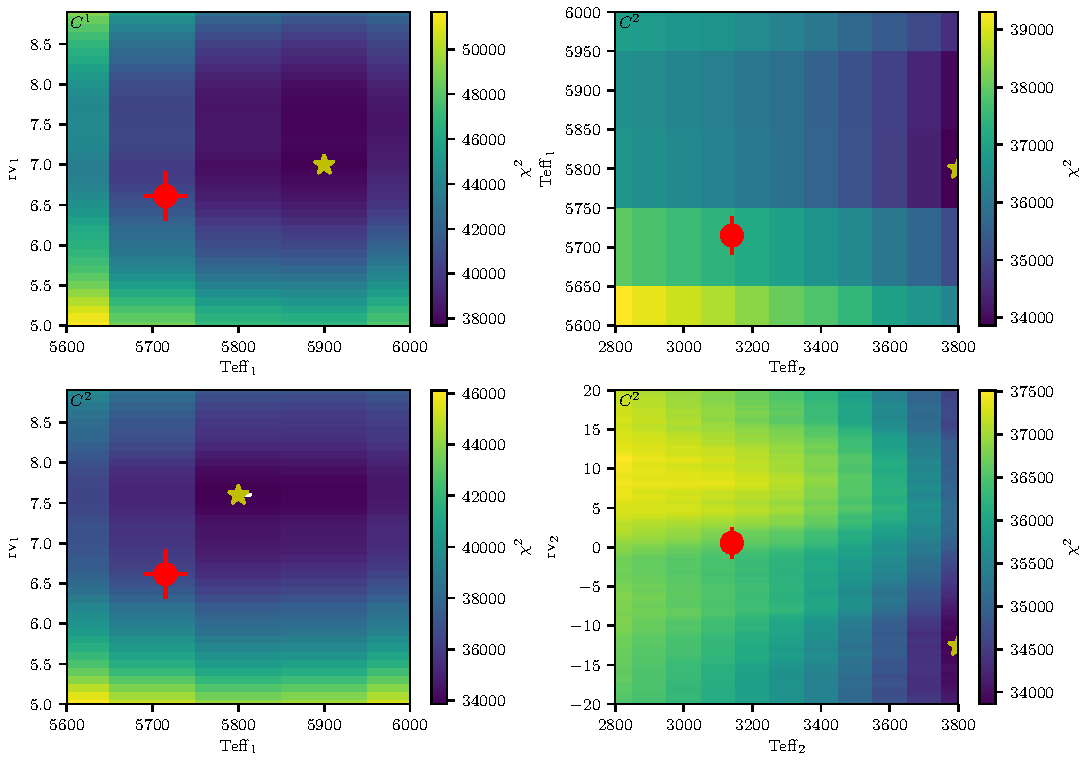
\includegraphics[width=0.7\linewidth]{figures/companion_recovery/HD211847_result_pcolors}
    \caption[\textchisquared{} contour for an observation {HD 211847}.]{\textchisquared{} result grid for observation 2 of {HD 211847}, similar to \cref{fig:Mdwarf_contours,fig:HD211847_simulated_contours}.
        The top right plot shows the application of a single component model (\(C^1\)) while the other three are using a binary model (\(C^2\)).
        Both left hand panels show the distribution of host temperature and host {RV}.\@ The top right panel shows the distribution for host and companion temperature, and the bottom right the companion temperature and radial velocity.
        The red circles indicate the literature values or calculated parameters for the target while the yellow star indicates the minimum \textchisquared{} solution.
        The error bar on the \(\teffsub{1}\) is from the literature while the error bars on \({rv}_{1}\) and \({rv}_{2}\) are calculated by propagating the orbital parameter uncertainties though the radial velocity equation.
        The white line shows a 3-\(\sigma\) confidence level about the minimum \textchisquared{} solution grid point, not always visible here due to the large \textchisquared{} values.}
    \label{fig:HD211847_result_contours}
\end{figure*}

\todo{Put error paragraph in a good location}
The error on estimated {RV} values, shown in \cref{fig:HD211847_result_contours}, is calculated by applying the general error propagation formula~\citep{ku_notes_1966} to the {RV} equation (\cref{eqn:rv2_equation}) and using the errors on the published orbital parameters.
For a function, \(f\), with errors on the inputs \(\delta x\), \(\delta y\) etc., it follows:
\begin{align}
f &= f(x, y, z, \ldots)\\
\delta f &= \sqrt{{\left( \frac{\partial f}{\partial x} \delta x\right)}^2 + {\left(\frac{\partial f}{\partial y} \delta y\right)}^2 + {\left(\frac{\partial f}{\partial z} \delta z\right)}^2 + \ldots}.
\end{align}


\begin{figure*}
    \centering
    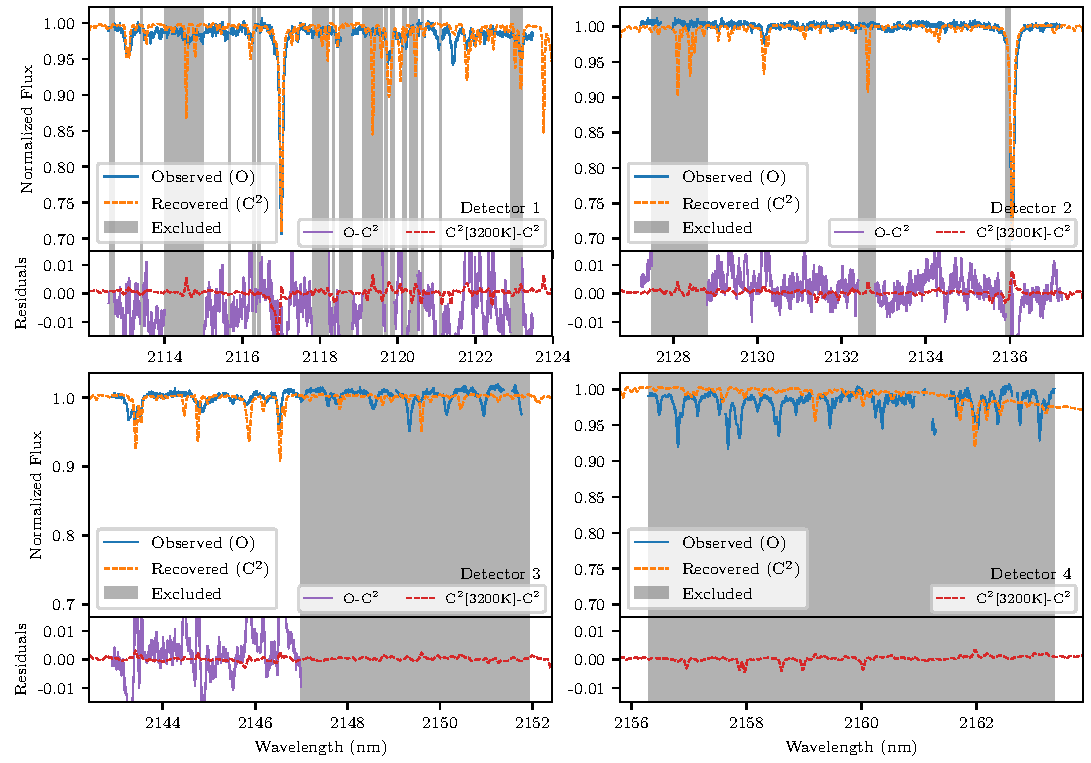
\includegraphics[width=0.7\linewidth]{figures/companion_recovery/visualize_result_residuals}
    \caption[Comparison between observation of {HD 211847} and the best fit synthetic binary model.]{Comparison between the observed {HD 211847} spectrum (blue) and the best fit synthetic binary model (orange dashed) for each detector.
        The bottom section of each panel shows the residuals between the parts of the observation used in the \textchisquared{} fit and recovered binary model (\(\rm O-C^2\)) in purple.
        The red dashed line shows the difference between the recovered binary model and the binary model with the exact same parameters except for the estimated companion temperature of 3200\K{} (\(\rm C^2[3200\K{}]- C^2\)).
        The grey shading indicated the wavelength regions where masking has been applied.
        The thinner masked regions that match with cuts in the observed spectra are where the centres of deep (>5\%) telluric lines that have been masked out are.}
    \label{fig:visualinspection-hd2118471}
    %\label{fig:visualizeresultresiduals}
\end{figure*}

